\documentclass[journal]{IEEEtran}
\usepackage{graphicx,amsmath,amssymb,booktabs,url,xcolor}
\usepackage{algorithm}
\usepackage{algpseudocode}
\usepackage{tikz}
\usetikzlibrary{arrows.meta,positioning,fit,backgrounds}
\usepackage[hidelinks]{hyperref}
\newcommand{\auroc}{\textsc{auroc}}
\newcommand{\bz}{\{0,1\}}

\begin{document}
\title{Logic-Aware Graph Neural Networks Predict
Asynchronous Reachability in Boolean
Gene-Regulatory Networks and Transfer Zero-Shot
to Real Networks}

\author{Kun~Zhang%
\thanks{K.~Zhang is with the University of Leeds, Leeds, U.K.
(e-mail: pjdf0740@leeds.ac.uk).}%
\thanks{Manuscript prepared June 2026. Code, synthetic generators, trained models, and
the symbolic label cache are publicly available at
\url{https://github.com/Beiciccc/attractornet}.}}

\markboth{IEEE/ACM Transactions on Computational Biology and Bioinformatics}%
{Zhang: Logic-Aware GNNs Predict Asynchronous Reachability in Boolean GRNs}

\maketitle

\begin{abstract}
Boolean networks (BNs) are a standard qualitative model of gene-regulatory and
signalling dynamics, in which the behaviour of interest is captured by attractors and
by reachability between states. Both are hard to compute exactly in general. Classical
theory connects a BN's interaction graph to its dynamics only through necessary
conditions and bounds, so the wiring diagram provably under-determines the attractor
set. We use this gap to pose a well-defined learning problem with free, exact
supervision. With an exact symbolic oracle supplying ground-truth labels, we first
measure the gap itself: a predictor restricted to graph topology performs at chance
(\auroc{} $0.56$), because fixing the wiring and varying only the Boolean functions
flips the attractor label for $84$--$88\%$ of wirings. We then introduce a sign-aware,
size-agnostic graph neural network (GNN) that reads the local Boolean logic and
predicts \emph{per-node asynchronous activation reachability}, that is, which genes can
switch on from a quiescent state. In distribution, the GNN beats a gradient-boosted
tree given \emph{all} truth-table bits on reachability ($0.96$ vs $0.92$), but not on
the more global has-cyclic property; we attribute this selective win to an inductive
bias rather than to capacity. Trained only on small synthetic BNs, the same GNN then
transfers \emph{zero-shot} to real curated gene-regulatory networks from the
biodivine-boolean-models collection, reaching pooled \auroc{} $0.91$ ($95\%$ CI
$[0.88,0.93]$) and outperforming every size-agnostic baseline, including a CANA
effective-connectivity baseline whose local-feature mapping fails to transfer. A
sign\,/\,no-sign\,/\,MLP ablation traces the gain to sign-aware message passing rather
than to recomputed canalization. Because all labels come from exact symbolic
computation, the method needs no manual annotation and runs on a single GPU.
\end{abstract}

\begin{IEEEkeywords}
Boolean networks, gene regulatory networks, graph neural networks, attractors,
asynchronous reachability, canalization, machine learning, systems biology.
\end{IEEEkeywords}

\section{Introduction}
\IEEEPARstart{H}{ow} much of a gene-regulatory network's long-run behaviour is fixed
by its \emph{wiring}, and how much by the regulatory \emph{logic} on that wiring?
Boolean networks (BNs) are a canonical qualitative model of gene regulation,
signalling, and cell-fate decision-making: each gene is a binary node, and a Boolean
update function of its regulators encodes the combinatorial logic of activation and
repression~\cite{kauffman,thomasoriginal}. The biologically meaningful predictions of
a BN are its \emph{attractors}, the long-run cyclic or steady patterns identified
with cell phenotypes, together with its \emph{reachability} structure: from a given
state, which configurations and which individual gene activations the dynamics can
attain. A question that recurs across systems biology is which genes can be switched on
from a quiescent (all-OFF) state, and by what regulatory routes. It underlies
reprogramming and signal-response analysis.

On the structural side the theory is sharp. Thomas's rules tie multistationarity to
positive feedback circuits and sustained oscillation to negative
circuits~\cite{richard2007,thomasreview}; Aracena bounds the number of fixed points by
the positive feedback vertex set~\cite{aracena2008}. Yet these are \emph{necessary
conditions and bounds} rather than determinations. The same signed interaction graph
admits update functions with one attractor or with many, and deciding the count from
the graph alone is \#P-complete~\cite{pcomplete}. The interaction graph, in short, does
not fix the dynamics; the logic does.

This under-determination is what turns prediction into a genuine \emph{learning}
problem (Fig.~\ref{fig:pipeline}). If the graph does not determine the dynamics, then a
model reading the graph alone can do no better than chance, and any model that succeeds
must be drawing on the \emph{logic}. Predicting a dynamical property from structure and
logic together is therefore a well-posed supervised task, with a built-in
identifiability guarantee and a free, exact label source in the symbolic oracle, and
with no need for manual annotation. We instantiate it for \emph{asynchronous
reachability}. This property is PSPACE-hard to compute exactly in general, it is
biologically central, and, unlike the mere existence of attractors, it is fundamentally
a \emph{propagation} phenomenon.

Our learner is a sign-aware, size-agnostic GNN that reads each node's local Boolean
function (through arity-invariant descriptors) and the signed wiring, and predicts
per-node activation reachability. Being size-agnostic, it is trained once on cheap
small synthetic networks and applied to real gene-regulatory networks (GRNs) it never
saw.

\noindent\textbf{Contributions.}
\begin{itemize}
\item \emph{An identifiability control.} An exact-oracle, de-confounded quantification
that the interaction graph under-determines BN attractor properties on our
distribution ($84$--$88\%$ label flips under fixed wiring; topology-only \auroc{}
$0.56$), certifying that a learned signal must come from the logic
(\S\ref{sec:identifiability}).
\item \emph{A logic-aware, sign-aware, size-agnostic GNN} predicting asynchronous
reachability that, in distribution, beats a gradient-boosted tree given \emph{all}
truth-table bits specifically on reachability and not on the global has-cyclic
property; this reflects an inductive bias rather than raw capacity. A sign\,/\,no-sign\,/\,MLP ablation and
a dedicated CANA effective-connectivity baseline isolate sign-aware propagation as the
source of the gain (\S\ref{sec:method},~\S\ref{sec:ablation}).
\item \emph{Zero-shot transfer to real GRNs.} Trained only on synthetic BNs, the GNN
predicts per-node activation reachability on real biodivine-boolean-models networks at
pooled \auroc{} $0.91$ ($95\%$ CI $[0.88,0.93]$), beating size-agnostic feature
baselines by ${+}0.08$ and a CANA baseline by ${+}0.45$ (\S\ref{sec:transfer}).
\item \emph{A reproducible, annotation-free pipeline}: an exact state-transition-graph
oracle for synthetic networks and symbolic BDD reachability for real ones, on a single
GPU.
\end{itemize}

\section{Background}
\label{sec:background}
\textbf{Boolean networks.} A BN on $n$ nodes assigns each node $i$ a Boolean update
function $f_i:\bz^{k_i}\!\to\!\bz$ of its $k_i$ \emph{regulators}. A global state is
$x\in\bz^n$. The \emph{signed interaction graph} has an edge $j\!\to\!i$ whenever $f_i$
depends on $x_j$; the edge is labelled $+$ ($-$) if $f_i$ is locally monotone
increasing (decreasing) in $x_j$, and unsigned if non-monotone. The graph thus records
\emph{who regulates whom and with what sign}, but discards the combinatorial logic of
how regulators combine.

\textbf{Updating schemes and attractors.} Under \emph{synchronous} update all nodes
update simultaneously, $x\mapsto F(x)=(f_1(x),\dots,f_n(x))$; the dynamics is a
deterministic functional graph whose cycles are the synchronous \emph{attractors}
(fixed points have period $1$). Under \emph{asynchronous} update one node updates at a
time, yielding a non-deterministic state-transition graph (STG) whose terminal
strongly connected components are the asynchronous attractors. Asynchronous update is
the more biologically faithful regime, avoiding artificial synchrony, but its STG has
out-degree up to $n$ and reachability questions are correspondingly harder (PSPACE-hard
in general).

\textbf{Reachability.} The \emph{forward-reachable set} of a state $x$ under
asynchronous dynamics is the set of states attainable by any sequence of single-node
updates. We focus on \emph{per-node activation reachability}: starting from the all-OFF
state $\mathbf 0$, can node $v$ ever take value $1$? Biologically this asks which genes
are activatable from quiescence; it is a node-classification target and is governed by
whether activation can \emph{propagate} along the signed wiring.

\textbf{Canalization.} A Boolean function is canalizing when some input value alone
fixes the output; nested canalization and the associated \emph{effective connectivity}
$k_e$ and \emph{input redundancy} measure how few inputs effectively
matter~\cite{cana}. Real GRN functions are strongly canalizing, which shapes their
dynamics; we therefore treat canalization features as a strong baseline to beat
(\S\ref{sec:ablation}).

\textbf{Why this is a learning problem.} Counting fixed points is \#P-complete and the
interaction graph only bounds it~\cite{aracena2008,pcomplete}; the graph
under-determines attractors and reachability (\S\ref{sec:identifiability}). Hence
predicting these properties from structure-plus-logic is non-trivial precisely where
the graph is uninformative. We emphasize that our aim is \emph{not} to replace the exact
symbolic solver on a speed basis (on the curated networks studied here the symbolic
oracle is itself fast), but to establish that the logic carries \emph{transferable}
reachability structure: a single learned model generalizes across networks it never
saw, whereas an exact solver must recompute each network from scratch and learns
nothing portable.

\section{Related Work}
\textbf{Structure$\to$dynamics theory.} Thomas's conjectures are proved by Richard and
Comet~\cite{richard2007} and are necessary, not sufficient; the same signed graph
supports very different dynamics depending only on the logic~\cite{thomasreview}.
Aracena bounds the fixed-point count by $2^{\tau^+}$~\cite{aracena2008}; deciding
$k$-fixed-points from the digraph is \#P-complete~\cite{pcomplete}, and the regulatory
logic, not the wiring, shapes the state-transition graph~\cite{sil2024}. We quantify
this gap as a control; we do not claim it as new.

\textbf{Predicting BN dynamics.} Rumiantsau \emph{et al.}~\cite{spectral2023} predict
BN attractors from structure via spectral analysis, which is non-learned and targets fixed-point
patterns, with no asynchronous reachability and no transfer. Weidner \emph{et
al.}~\cite{weidner2021} rank node dynamic-impact from graph-theoretic features (a
forest on graph measures); this is exactly our topology baseline, which we show is
near-chance for reachability. GATTACA~\cite{gattaca} pairs a GNN with reinforcement
learning for cellular-reprogramming \emph{control}, but \emph{assumes} attractors are
pre-computed by a separate procedure, a different task in which the dynamics are handed to
the model rather than predicted. To our knowledge, no prior work learns to predict
asynchronous reachability of BNs from local logic, and none demonstrates
synthetic$\to$real transfer.

\textbf{Learning discrete dynamics; canalization.} Methods that learn \emph{unknown}
local rules from observed trajectories~\cite{arnca} address the inverse,
system-identification problem and do not read a known Boolean logic; ML for ``Boolean
control network reachability'' is uniformly reinforcement-learning \emph{control}; and
ML for GRNs is overwhelmingly network \emph{inference} (the opposite direction to
forward dynamics prediction). The strongest non-trivial baseline is canalization:
effective connectivity and input redundancy (CANA)~\cite{cana} are known local logic
features that strongly shape BN dynamics; \S\ref{sec:ablation} shows our gain is not
recomputed canalization.

\textbf{Data and oracle.} We use the biodivine-boolean-models (BBM) collection of
curated biological BNs, with exact attractor/reachability analysis from
\texttt{biodivine\_aeon} and \texttt{biobalm} (symbolic, BDD-based)~\cite{aeon,aeoncav,biobalm},
repurposed here as a zero-cost supervision source.

\begin{figure}[t]
\centering
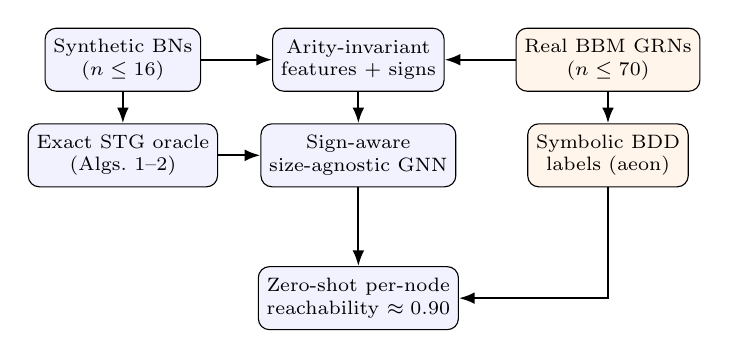
\begin{tikzpicture}[
  font=\scriptsize,
  box/.style={draw,rounded corners,align=center,inner sep=3pt,minimum height=8mm,fill=blue!5},
   db/.style={draw,rounded corners,align=center,inner sep=3pt,minimum height=8mm,fill=orange!8},
  arr/.style={-{Latex[length=2mm]},thick}]
\node[box] (syn) {Synthetic BNs\\($n\le16$)};
\node[box,below=4mm of syn] (oracle) {Exact STG oracle\\(Algs.~1--2)};
\node[box,right=9mm of syn] (feat) {Arity-invariant\\features + signs};
\node[box,below=4mm of feat] (gnn) {Sign-aware\\size-agnostic GNN};
\node[db,right=9mm of feat] (real) {Real BBM GRNs\\($n\le70$)};
\node[db,below=4mm of real] (bdd) {Symbolic BDD\\labels (aeon)};
\node[box,below=10mm of gnn] (pred) {Zero-shot per-node\\reachability $\approx0.90$};
\draw[arr] (syn)--(oracle);
\draw[arr] (syn)--(feat);
\draw[arr] (oracle.east)-- ++(2mm,0) |- (gnn.west);
\draw[arr] (feat)--(gnn);
\draw[arr] (real)--(bdd);
\draw[arr] (real.west)-- ++(-2mm,0) |- (feat.east);
\draw[arr] (gnn)--(pred);
\draw[arr] (bdd.south) |- (pred.east);
\end{tikzpicture}
\caption{Pipeline. An exact state-transition-graph oracle labels small synthetic BNs;
a sign-aware, size-agnostic GNN trained on their logic transfers zero-shot to real GRNs
labelled by symbolic BDD reachability.}
\label{fig:pipeline}
\end{figure}

\section{Tasks and the Exact Oracle}
\label{sec:tasks}
\textbf{Prediction tasks.} We study three exact-oracle labels: (a)
\emph{has-cyclic-attractor}, whether a synchronous attractor of period $>1$ exists; (b)
\emph{attractor count}; and (c), our headline task, \emph{per-node activation
reachability} as defined in \S\ref{sec:background}. Tasks (a)--(b) are global
network-level properties; task (c) is node-level and propagation-structured.

\textbf{Synthetic oracle.} For small networks ($n\le16$) we compute labels exactly by
enumerating the STG. Synchronous attractors are the cycles of the functional graph
(Alg.~\ref{alg:sync}), found by a single colour-marked traversal in $O(2^n)$ time.
Per-node activation reachability is computed by an asynchronous breadth-first search
from $\mathbf 0$, OR-accumulating all reachable states (Alg.~\ref{alg:reach}); node $v$
is labelled $1$ iff bit $v$ is set in the accumulated reachable set. Both are exact and
deterministic.

\begin{algorithm}[t]
\caption{Exact synchronous attractors}
\label{alg:sync}
\begin{algorithmic}[1]
\State $\mathrm{succ}[s]\gets F(s)$ for all $s\in\bz^n$; $\mathrm{col}\gets 0$
\For{$s_0\in\bz^n$ with $\mathrm{col}[s_0]=0$}
  \State follow successors marking $\mathrm{col}=1$ until a marked state $s$ is hit
  \If{$s$ is on the current path} record the cycle $s\!\to\!\dots\!\to\!s$ \EndIf
  \State mark the whole path $\mathrm{col}=2$
\EndFor
\State \Return list of cycles (attractors); period $1\Rightarrow$ fixed point
\end{algorithmic}
\end{algorithm}

\begin{algorithm}[t]
\caption{Per-node activation reachability (async, from $\mathbf 0$)}
\label{alg:reach}
\begin{algorithmic}[1]
\State $\mathrm{seen}\gets\{\mathbf 0\}$; $Q\gets[\mathbf 0]$; $r\gets\mathbf 0$
\While{$Q$ non-empty}
  \State $s\gets Q.\mathrm{pop}()$
  \For{$i=1\dots n$ with $f_i(s)\neq s_i$}
    \State $s'\gets s$ with bit $i$ flipped
    \If{$s'\notin\mathrm{seen}$} add $s'$ to $\mathrm{seen},Q$; $r\gets r\,|\,s'$ \EndIf
  \EndFor
\EndWhile
\State \Return label$[v]=r_v$ for each node $v$
\end{algorithmic}
\end{algorithm}

\textbf{Real-network oracle.} For real networks explicit STG enumeration is infeasible,
so we use \texttt{biodivine\_aeon}'s symbolic, binary-decision-diagram (BDD) forward
reachability, which represents reachable sets compactly and scales beyond $2^n$ for
structured networks~\cite{aeon}. Real BBM models contain \emph{external-input} nodes
(no regulators, a free signal); we fix these to OFF, consistent with the all-OFF
quiescent initial condition, so that reachability is deterministic and per-node labels
are well defined. We then compute, per gene $v$, whether $v=1$ is in the forward-reachable
set from quiescence.

\textbf{Datasets and coverage.} Synthetic training data are exact-labelled small BNs
($n\in\{12,14\}$, in-degree $K\in\{2,3,4\}$, random and nested-canalizing logic). For
real evaluation we draw from the $285$ curated BBM networks; after fixing inputs and
keeping fully-specified networks with $n\le70$, $178$ are labelled successfully
(symbolic labelling is process-isolated with a hard timeout; $4$ time out, $4$ are
parameterized), of which $118$ have class variance and are used for \auroc{}
(Table~\ref{tab:coverage}).

\begin{table}[t]
\caption{Real-network (BBM) coverage for evaluation.}
\label{tab:coverage}
\centering
\begin{tabular}{lc}
\toprule
quantity & value\\
\midrule
curated BBM networks & $285$\\
fully-specified, $n\le70$, labelled & $178$\\
\ \ with class variance (used for \auroc{}) & $118$\\
labelled nodes (class-varying nets) & $3659$\\
activation base rate (pooled) & $0.34$\\
skipped: parameterized\,/\,timeout & $4\,/\,4$\\
\bottomrule
\end{tabular}
\end{table}

\section{Identifiability: the graph under-determines the dynamics}
\label{sec:identifiability}
Graph under-determination is established theory (\S\ref{sec:background}); we present a
quantitative, de-confounded version solely as an identifiability control that makes the
learning problem well-posed, certifying that any signal our GNN extracts comes from the
logic rather than the wiring.

\textbf{Design.} We generate $480$ fixed-wiring families ($n\in\{12,14\}$,
$K\in\{2,3,4\}$) and draw $8$ logic variants (random and nested-canalizing) per family
on the \emph{same} wiring, labelling each exactly. A \emph{within-graph} split places
different logic variants of the same wirings in train and test. One detail matters here:
we \emph{balance} the random/canalizing mix across the split, because a naive variant-parity split
inadvertently trains on all-random and tests on all-canalizing logic, leaking a
distribution shift that artificially depresses scores. Balancing removes this confound.

\textbf{Results.} Holding the wiring fixed and varying only the logic flips the label
for $84\%$ of wirings (has-cyclic) and $88\%$ (reachability). On these instances,
any topology-only predictor is, by construction, near-chance. Empirically a topology
predictor reaches \auroc{} $0.558$, a shuffle-label null $0.52$
(Table~\ref{tab:identify}, Fig.~\ref{fig:learn}a). The signed graph (Thomas level) helps for
has-cyclic ($0.86$) but remains at chance for reachability ($0.566$); only features
that read the logic predict reachability ($0.92$). Thus the logic, not the wiring,
carries the reachability signal.

\textbf{Not merely chaos.} One might worry the learnable residual is just the
Kauffman--Derrida order--chaos transition. Table~\ref{tab:chaos} controls for this: the
structural/logic features beat the mean-field sensitivity $\lambda$ (the Derrida slope)
by ${+}0.07$ \auroc{}, and in the ordered regime ($K=1$) structure predicts the
attractor count ($R^2=0.73$) where $\lambda$ alone is uninformative ($R^2=-0.05$). The
learnable signal is genuine logic-dependent structure, not the chaos order parameter.

\begin{table}[t]
\caption{Within-graph \auroc{} by feature group (de-confounded).}
\label{tab:identify}
\centering
\begin{tabular}{lcc}
\toprule
feature group & has-cyclic & async reachability\\
\midrule
topology (wiring only) & $0.558$ & $0.558$\\
signed graph (Thomas) & $0.860$ & $0.566$\\
logic-aware (all truth-table bits) & $0.803$ & $0.921$\\
shuffle-label null & $0.520$ & $0.515$\\
\bottomrule
\end{tabular}
\end{table}

\begin{table}[t]
\caption{Chaos control: structure vs.\ the Derrida sensitivity $\lambda$.}
\label{tab:chaos}
\centering
\begin{tabular}{lcc}
\toprule
predictor & has-cyclic \auroc{} & count $R^2$ ($K{=}1$)\\
\midrule
$\lambda$ alone (Derrida) & $0.799$ & $-0.045$\\
structural / logic features & $0.872$ & $0.727$\\
gain beyond $\lambda$ & $+0.073$ & $+0.772$\\
\bottomrule
\end{tabular}
\end{table}

\begin{figure*}[t]
\centering
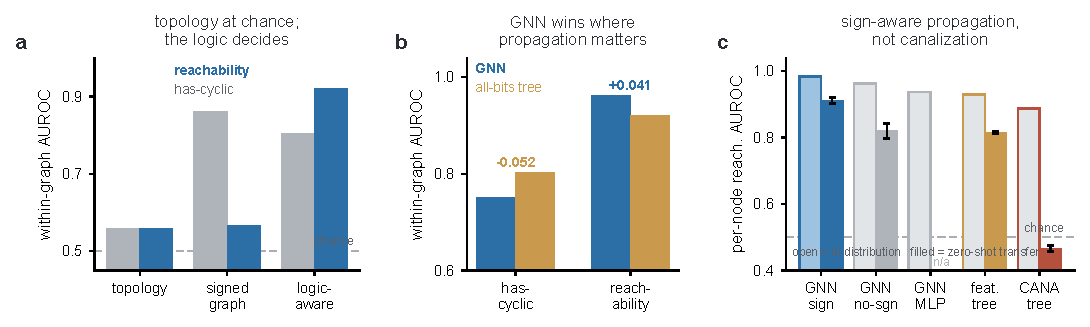
\includegraphics[width=0.99\textwidth]{fig_composite_learn.pdf}
\caption{The logic, not the wiring, carries learnable reachability structure.
\textbf{a}, Within-graph \auroc{} by feature group (de-confounded): topology is at
chance for both tasks, the signed graph helps only has-cyclic, and only logic-aware
features predict reachability. \textbf{b}, The GNN's advantage is task-specific: it
beats the all-bits tree on asynchronous reachability (propagation-shaped) but loses on
the global has-cyclic property. \textbf{c}, Sign-aware propagation, not canalization:
in-distribution (open bars) and zero-shot transfer (filled bars) \auroc{} for the GNN
variants and the canalization baselines; the GNN-sign model (blue) stays high on
transfer while the CANA tree drops below chance. Error bars: std over $3$ seeds.}
\label{fig:learn}
\end{figure*}

\section{Method}
\label{sec:method}
\textbf{Arity-invariant node features.} Each node is described by features defined for
\emph{any} in-degree, so the same encoder applies to synthetic nodes of in-degree $4$
and real nodes of in-degree $15$ (Table~\ref{tab:feats}). None is a fixed-width truth
table; for high-arity real nodes the function-derived features (bias, sensitivity,
canalizing depth) are estimated by sampling, keeping per-node cost bounded.

\begin{table}[t]
\caption{Arity-invariant per-node features.}
\label{tab:feats}
\centering
\begin{tabular}{ll}
\toprule
group & features\\
\midrule
degree & in-degree, out-degree\\
function bias & mean output $\Pr[f{=}1]$\\
canalization & canalizing depth (\#\,canalizing inputs)\\
sensitivity & mean and max single-input activity\\
edge signs & fractions activating / inhibiting / non-monotone\\
\bottomrule
\end{tabular}
\end{table}

\textbf{Sign-aware message passing.} We separate incoming edges by sign and learn
distinct transforms for positive and negative regulators. With $A^{+},A^{-}$ the
positive/negative signed adjacency (mean-normalized, $\widehat{\cdot}$) and $H^{(\ell)}$
the layer-$\ell$ node states,
\begin{equation}
H^{(\ell+1)} = \sigma\!\big(W_s H^{(\ell)} + W_p\,\widehat{A^{+}}H^{(\ell)} +
W_n\,\widehat{A^{-}}H^{(\ell)}\big).
\label{eq:mp}
\end{equation}
Eq.~\eqref{eq:mp} is a standard relational/signed message-passing layer in the style of
R-GCN~\cite{rgcn} and signed graph convolution~\cite{signedgcn}, with the two relations
being positive and negative regulation; we do not claim the architecture itself as novel.
Our contribution is the \emph{task framing} (predicting logic-dependent reachability where
the graph is provably uninformative) and the \emph{zero-shot synthetic$\to$real transfer},
for which a sign-aware encoder is the natural choice and, as the ablation shows, a
decisive one. We use
three layers ($64$ hidden units) and a per-node sigmoid head (Alg.~\ref{alg:gnn}),
implemented as sparse edge-list message passing (scatter-add) so it runs on networks of
any size (trained at $n\le16$, applied to $n$ up to hundreds). Separating sign is
biologically motivated: whether activation propagates to a node depends on whether its
regulators activate or inhibit it, information that a sign-agnostic aggregator discards. The
ablation in \S\ref{sec:ablation} confirms that this term is doing the work.

\begin{algorithm}[t]
\caption{Sign-aware GNN forward pass (per-node head)}
\label{alg:gnn}
\begin{algorithmic}[1]
\State $H\gets\mathrm{ReLU}(W_\text{in}X)$ \Comment{$X$: arity-invariant features}
\For{$\ell=1\dots L$}
  \State $M^+\!\gets\!\widehat{A^+}H,\;M^-\!\gets\!\widehat{A^-}H$ \Comment{sign-split mean aggregation}
  \State $H\gets\mathrm{ReLU}(W_s H + W_p M^+ + W_n M^-)$
\EndFor
\State \Return $\sigma(W_\text{out}H)$ \Comment{per-node activation probability}
\end{algorithmic}
\end{algorithm}

\textbf{Baselines.} We compare against three baselines, in increasing strength.
\emph{Flat-TT}: a gradient-boosted tree on the concatenation of \emph{all} node
truth-table bits plus the signed wiring, an upper bound on the logic information
available, but applicable only at a fixed small size. \emph{Feature tree}: a
gradient-boosted tree on the same size-agnostic arity-invariant features the GNN uses
(without the graph structure). \emph{CANA tree}: a gradient-boosted tree on a full
CANA-style canalization suite: per-input activity, effective connectivity $k_e$, input
redundancy, activity distribution, canalizing depth, bias (\S\ref{sec:ablation}). The
last directly tests whether the GNN merely recomputes canalization.

\textbf{Training.} The GNN is trained with binary cross-entropy (Adam, lr $2\times
10^{-3}$, weight decay $10^{-5}$, $60$ epochs) on the synthetic node set; no real-network
labels are used in training. All results are mean$\pm$std over $3$ training seeds.

\section{Experiments}
\textbf{Setup.} Synthetic training and the $118$-network real test set are as in
\S\ref{sec:tasks} (Table~\ref{tab:coverage}). We evaluate \auroc{} for the binary tasks.

\subsection{In-distribution and the inductive-bias result}
On the de-confounded within-graph split the flat-TT tree, which has \emph{all} the
logic bits, reaches $0.803$ (has-cyclic) and $0.921$ (reachability), far above the
$0.52$ null and generalizing leave-graph-out ($0.819/0.916$). The GNN beats the flat-TT
tree on \emph{reachability} ($0.962$ vs $0.921$) but \emph{loses} on the global
\emph{has-cyclic} property ($0.751$ vs $0.803$, Fig.~\ref{fig:learn}b). A win on one task
and a loss on the other points to an inductive bias rather than to greater capacity:
message passing captures the propagation structure of reachability, whereas a
feature-interaction tree does as well or better on a property that is not
propagation-shaped. The GNN is therefore suited specifically to reachability.


\subsection{Zero-shot transfer to real GRNs}
\label{sec:transfer}
We train the per-node reachability predictor on synthetic networks only, convert each
real BBM network to the same representation, and evaluate zero-shot. The headline metric
is the pooled \auroc{} over all $3659$ nodes of the $118$ real GRNs, with a
\emph{cluster} bootstrap that resamples whole networks ($2000$ replicates) to respect
within-network correlation. The size-agnostic GNN attains pooled \auroc{}
$\mathbf{0.906}$, $95\%$ CI $[0.879,0.932]$, versus $0.816$ $[0.794,0.836]$ for the
size-agnostic feature tree; the paired difference is $+0.091$, $95\%$ CI
$[0.064,0.116]$, which excludes zero. The per-net \auroc{} distribution is right-skewed
(median $0.99$, IQR $[0.85,1.00]$, mean $0.90$; Fig.~\ref{fig:transfer}a); we report the pooled
mean as the headline and the median only as a descriptor of the typical network. The
flat-TT tree is \emph{inapplicable} at these sizes (variable $n$ and arity), and exact
solvers do not generalize; they recompute per network.

\textbf{Failure analysis.} $12$ of $118$ networks fall below \auroc{} $0.7$. Contrary to
what one might guess, this tail is \emph{not} explained by size: $10/12$ have $n\ge15$,
the median tail size is $21$, the worst case is $n=28$ (\auroc{} $0.222$), and across all
$118$ networks per-net \auroc{} is essentially uncorrelated with size (Spearman
$\rho=-0.14$, $p=0.14$; Fig.~\ref{fig:transfer}a, left). The tail instead comprises networks whose
wiring or sign structure is atypical relative to the synthetic training distribution;
characterizing these hard cases precisely is left to future work.

\begin{figure*}[t]
\centering
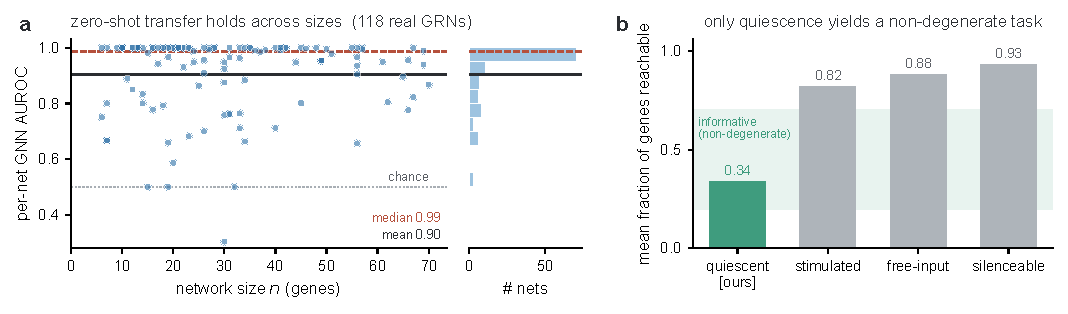
\includegraphics[width=0.99\textwidth]{fig_composite_transfer.pdf}
\caption{Zero-shot transfer to real GRNs, and why the quiescent task is principled.
\textbf{a}, Per-net \auroc{} of the synthetic-trained GNN on the $118$ real BBM
networks vs network size (left), with the right-skewed distribution (right; median
$0.99$, mean $0.90$); transfer is stable across sizes. \textbf{b}, Mean fraction of
genes reachable under four driving conditions: only the quiescent inputs-OFF task we
study (green) avoids saturation and falls in the informative band, so it is the
principled non-degenerate choice rather than a cherry-picked one.}
\label{fig:transfer}
\end{figure*}

\subsection{The gain is sign-aware propagation, not canalization}
\label{sec:ablation}
One might object that reachability is already recoverable from known \emph{local} logic
features such as canalization and effective connectivity, so that the transfer result
merely exploits the fact that real GRNs are heavily canalizing. Two experiments argue
against this reading (Table~\ref{tab:ablation},
Fig.~\ref{fig:learn}c).

First, an ablation of three GNN variants: \emph{sign} (separate $\pm$ transforms),
\emph{no-sign} (message passing, sign ignored), and \emph{MLP} (no message passing, a
neural model on the per-node features, i.e.\ a neural canalization baseline). In
distribution, message passing adds ${+}0.026$ over the MLP and sign-awareness a further
${+}0.021$; on real GRNs the effect sharpens: sign-awareness adds ${+}0.093$, with the
sign-agnostic GNN collapsing to the feature-baseline level. Propagation, and the sign of
regulation, are what the GNN exploits.

Second, a dedicated CANA effective-connectivity tree~\cite{cana}: per-input activity
$a_i=\Pr_x[f(x)\neq f(x\oplus e_i)]$, effective connectivity $k_e=\sum_i a_i$, input
redundancy $r=1-k_e/k$, the activity distribution, canalizing depth, and bias. The GNN
beats this strengthened baseline by ${+}0.097$ in distribution; on transfer the CANA
tree drops to \auroc{} $0.465$, slightly below chance. We read the below-chance value not
as evidence that canalization is irrelevant to the dynamics (it is not), but as a
\emph{distribution-shift artifact}: the local canalization$\to$activatability relation
learned on the synthetic ensemble inverts on real GRNs, so a model relying only on those
local features fails to port. The substantive comparison is therefore the in-distribution
gap ($+0.097$, where no shift confounds it) together with the sign\,/\,no-sign ablation,
which jointly indicate that the GNN's \emph{transferable} signal is sign-aware propagation
rather than a re-encoding of local canalization.

\begin{table}[t]
\caption{Per-node activation reachability: the GNN vs canalization baselines
(mean$\pm$std over $3$ training seeds). The sign-aware transfer figure here
($0.911$) is consistent with the network-level cluster-bootstrap headline of
\S\ref{sec:transfer} ($0.906$, $95\%$ CI $[0.879,0.932]$); the two harnesses differ
only in synthetic-training budget.}
\label{tab:ablation}
\centering
\begin{tabular}{lcc}
\toprule
method & in-distribution & transfer (real)\\
\midrule
GNN (sign-aware) & $\mathbf{0.984\pm0.001}$ & $\mathbf{0.911\pm0.010}$\\
GNN (sign-agnostic) & $0.963\pm0.002$ & $0.820\pm0.022$\\
GNN (MLP, no msg.\ passing) & $0.937\pm0.002$ & ---\\
feature tree & $0.929\pm0.003$ & $0.814\pm0.003$\\
CANA effective-connectivity tree & $0.887\pm0.002$ & $0.465\pm0.009$\\
\bottomrule
\end{tabular}
\end{table}


\subsection{Controls}
Beyond the chaos control (Table~\ref{tab:chaos}) and the shuffle-null and leave-graph-out
checks, we verify the reachability signal is not a trivial output-bias artifact
(Table~\ref{tab:trivial}): a mean-output-bias-only predictor reaches just $0.716$ versus
$0.921$ for the full model, and predictability persists ($0.897$) for a non-trivial
target state where a bias predictor is even weaker ($0.671$). All transfer splits are
de-confounded for the random/canalizing logic mix.

\begin{table}[t]
\caption{Trivial-bias control (reachability \auroc{}).}
\label{tab:trivial}
\centering
\begin{tabular}{lcc}
\toprule
predictor & all-ones target & non-trivial target\\
\midrule
mean-output-bias only & $0.716$ & $0.671$\\
full logic features & $0.921$ & $0.897$\\
\bottomrule
\end{tabular}
\end{table}

\subsection{Application: the budding-yeast cell cycle}
\label{sec:vignette}
To make the predictions concrete, we apply the synthetic-trained GNN \emph{zero-shot} to
the budding-yeast cell-cycle network, a classic Boolean GRN model in the BBM collection
($n=20$; source: \emph{PLoS ONE}, doi:10.1371/journal.pone.0045780), and ask which genes
are activatable from G1 quiescence (the all-OFF state). The predictor attains \auroc{}
$0.91$ over all $20$ genes (thresholded accuracy $0.70$, $14/20$ genes correct): it ranks
the core cyclins and regulators (Clb2, Clb5, Cdh1, Sic1, Whi5) as activatable and the
cell-size, spindle, and budding checkpoints (Size, SpindleCP, BuddingCP) and Cln2 as
\emph{not} spontaneously activatable from quiescence (Table~\ref{tab:vignette}), which is qualitatively
consistent with cell-cycle entry requiring size and signal cues rather than arising
spontaneously. The errors are intermediate regulators near the activatable boundary
(e.g.\ Cdc20, Cln3, FEAR). This is an \emph{illustration} of the prediction, not an
independent validation: the labels here are themselves from the exact oracle, so the
vignette shows what the zero-shot predictor recovers on a familiar network rather than
establishing a new biological finding.

\begin{table}[t]
\caption{Zero-shot per-gene activation-reachability predictions on the budding-yeast
cell cycle (selected genes; \auroc{} $0.91$ over all $20$).}
\label{tab:vignette}
\centering
\begin{tabular}{lcc}
\toprule
gene & GNN $p$(activatable) & exact label\\
\midrule
Clb2 & $1.00$ & activatable\\
Clb5 & $1.00$ & activatable\\
Cdh1 & $1.00$ & activatable\\
Sic1 & $1.00$ & activatable\\
Whi5 & $1.00$ & activatable\\
\midrule
Cdc14 & $0.18$ & not\\
SpindleCP & $0.01$ & not\\
BuddingCP & $0.01$ & not\\
Start & $0.01$ & not\\
Cln2 & $0.00$ & not\\
\bottomrule
\end{tabular}
\end{table}

\section{Discussion and Limitations}
The GNN's advantage is \emph{task-specific}: it wins on reachability, the
propagation-shaped property, and not on the global has-cyclic property
(\S\ref{sec:transfer}); we do not claim a universal dynamics predictor, and view the
match between message-passing locality and reachability propagation as the explanation.
Per-node reachability difficulty depends strongly on the \emph{driving condition}, and
the quiescent activation task we study is the principled non-degenerate choice rather
than a hand-picked one. We verified this on the real BBM networks: the all-OFF /
inputs-OFF convention is well-behaved (pooled base $0.34$), whereas the natural
alternatives all \emph{saturate} (Fig.~\ref{fig:transfer}b): a free-input ``activatable
under some signal'' variant (mean base $0.88$), a fully-stimulated condition (inputs
fixed ON; mean per-net base $0.82$), and a silenceability condition (reaching $0$ from
the all-ON state; mean base $0.93$) each make almost every gene reachable, leaving little
to predict. The quiescent condition is thus not cherry-picked for learnability but is the
one biologically meaningful condition that yields a non-degenerate label; characterizing
the framework under richer, non-saturating multi-signal conditions is important future
work.

There is a genuine synthetic$\to$real distribution shift (synthetic activation base rate
$0.86$ vs real $0.34$); the GNN transfers in spite of it, which is its main strength, although a
synthetic ensemble matched to GRN statistics (scale-free wiring, realistic
nested-canalizing prevalence) could shrink the shift and is promising future work.
Finally, exact synthetic ground truth limits training networks to $n\le16$. We stress
that on the curated networks studied here the symbolic oracle is fast (it labels almost
all of them in well under a second), so the contribution is a scientific one, namely
that the logic carries transferable reachability structure, rather than a computational speed-up; we
make no efficiency claim over the exact solver in this regime.

\section{Conclusion}
The wiring diagram is necessary but far from sufficient for a Boolean network's
dynamics. We have used that classical fact as the starting point for a well-posed
learning problem with free, exact supervision. A sign-aware, size-agnostic GNN that
reads the local logic predicts asynchronous reachability, and it beats an
all-truth-table-bits model exactly where propagation matters. Trained only on small
synthetic networks, the same model transfers zero-shot to real gene-regulatory networks
and outperforms every size-agnostic baseline, including a canalization model that does
not transfer at all. The logic, then, carries learnable and transferable reachability
structure that no graph-only model can recover, and a propagation-matched architecture
is what brings it within reach.

\section*{Reproducibility}
All labels are computed by exact symbolic tools (state-transition-graph enumeration;
\texttt{biodivine\_aeon} BDD reachability); no human annotation or external API is used.
The synthetic generators, the GNN, and all baselines run on a single GPU; the curated
networks are the public biodivine-boolean-models collection. All code, trained models,
and the symbolic label cache (sufficient to reproduce every reported number, including
the bootstrap CIs) are available at \url{https://github.com/Beiciccc/attractornet}.

\begin{thebibliography}{99}
\bibitem{kauffman} S. A. Kauffman, ``Metabolic stability and epigenesis in randomly
constructed genetic nets,'' \emph{J. Theor. Biol.}, vol. 22, no. 3, pp. 437--467, 1969.
\bibitem{thomasoriginal} R. Thomas, ``Boolean formalization of genetic control
circuits,'' \emph{J. Theor. Biol.}, vol. 42, no. 3, pp. 563--585, 1973.
\bibitem{richard2007} A. Richard and J.-P. Comet, ``Necessary conditions for
multistationarity in discrete dynamical systems,'' \emph{Discrete Appl. Math.}, vol.
155, no. 18, pp. 2403--2413, 2007.
\bibitem{thomasreview} A. Richard, ``Positive and negative cycles in Boolean networks,''
\emph{J. Theor. Biol.}, vol. 463, pp. 67--76, 2019.
\bibitem{aracena2008} J. Aracena, ``Maximum number of fixed points in regulatory
Boolean networks,'' \emph{Bull. Math. Biol.}, vol. 70, no. 5, pp. 1398--1409, 2008.
\bibitem{pcomplete} F. Bridoux, A. Durbec, K. Perrot, and A. Richard, ``Complexity of
fixed point counting problems in Boolean networks,'' \emph{J. Comput. Syst. Sci.}, vol.
126, pp. 138--164, 2022.
\bibitem{sil2024} P. Sil, A. Subbaroyan, S. Kulkarni, O. C. Martin, and A. Samal,
``Biologically meaningful regulatory logic enhances the convergence rate in Boolean
networks and bushiness of their state transition graph,'' \emph{Brief. Bioinform.}, vol.
25, no. 3, art. bbae150, 2024.
\bibitem{spectral2023} D. Rumiantsau, A. Lesne, and M.-T. H\"utt, ``Predicting
attractors from spectral properties of stylized gene regulatory networks,'' \emph{Phys.
Rev. E}, vol. 108, no. 1, art. 014402, 2023.
\bibitem{weidner2021} F. M. Weidner \emph{et al.}, ``Capturing dynamic relevance in
Boolean networks using graph-theoretical measures,'' \emph{Bioinformatics}, vol. 37, no.
20, pp. 3530--3537, 2021.
\bibitem{gattaca} A. Mizera and J. Zarzycki, ``The GATTACA framework: Graph neural
network-based reinforcement learning for controlling biological networks,'' in \emph{Proc.
AAAI Conf. Artif. Intell. (AAAI-26)}, vol. 40, no. 2, 2026, pp. 873--880.
\bibitem{arnca} B. Kang, H. Kumar, M. Lee, B. Chakraborty, and S. Mukhopadhyay,
``Learning locally interacting discrete dynamical systems: Towards data-efficient and
scalable prediction,'' in \emph{Proc. 6th Annu. Learn. Dyn. Control Conf. (L4DC)}, Proc.
Mach. Learn. Res., vol. 242, 2024, pp. 1357--1369.
\bibitem{cana} M. Marques-Pita and L. M. Rocha, ``Canalization and control in automata
networks: Body segmentation in \emph{Drosophila melanogaster},'' \emph{PLoS ONE}, vol. 8,
no. 3, art. e55946, 2013.
\bibitem{aeon} N. Bene\v{s}, L. Brim, O. Huvar, S. Pastva, D. \v{S}afr\'{a}nek, and E.
\v{S}mij\'{a}kov\'{a}, ``AEON.py: Python library for attractor analysis in asynchronous
Boolean networks,'' \emph{Bioinformatics}, vol. 38, no. 21, pp. 4978--4980, 2022.
\bibitem{aeoncav} N. Bene\v{s}, L. Brim, J. Kadlecaj, S. Pastva, and D. \v{S}afr\'{a}nek,
``AEON: Attractor bifurcation analysis of parametrised Boolean networks,'' in
\emph{Computer Aided Verification (CAV 2020)}, LNCS, vol. 12224. Springer, 2020, pp.
569--581.
\bibitem{biobalm} V.-G. Trinh, K. H. Park, S. Pastva, and J. C. Rozum, ``Mapping the
attractor landscape of Boolean networks with biobalm,'' \emph{Bioinformatics}, vol. 41,
no. 5, art. btaf280, 2025.
\bibitem{rgcn} M. Schlichtkrull, T. N. Kipf, P. Bloem, R. van den Berg, I. Titov, and M.
Welling, ``Modeling relational data with graph convolutional networks,'' in \emph{The
Semantic Web (ESWC 2018)}, LNCS, vol. 10843. Springer, 2018, pp. 593--607.
\bibitem{signedgcn} T. Derr, Y. Ma, and J. Tang, ``Signed graph convolutional networks,''
in \emph{Proc. IEEE Int. Conf. Data Mining (ICDM)}, 2018, pp. 929--934.
\end{thebibliography}

\end{document}
